% !TEX root = ../thesis.tex

\chapter{Vorherige Arbeit}
\label{ch:vorherige-arbeit}

Das Kernproblem der Arbeit lässt sich in drei verschiedene Teile gliedern:
Segmentierung in einzelne Cluster (\ref{sec:segmentation}), Registrierung von mehreren Punktwolken in einem Koordinatensystem (\ref{sec:registration}) und Triangulierung der Wolke zu einem Polygonnetz (\ref{sec:triangulation}).

Im Folgenden werden die wissenschaftlichen Erkenntnisse zum jeweiligen Thema erläutert.
Außerdem werden mögliche Lösungsansätze auf ihren praktischen Nutzen untersucht und die Vor- und Nachteile diskutiert.



\section{Segmentierung}
\label{sec:segmentation}

Ziel der Segmentierung ist es, zusammengehörende Bildregionen zu identifizieren und durch Zuweisung verschiedener Klassen voneinander zu trennen.
Dies ist, insbesondere in der 2D-Bildverarbeitung, ein lange bekanntes Problem, für das es viele verschiedene Lösungsansätze gibt.
Auch im dreidimensionalen Raum ist eine Segmentierung häufig notwendig.
In vielen Fällen gibt es dabei nicht eine beste Methode -- die Objektart, -größe, -form und viele weitere Faktoren beeinflussen die Wahl eines geeigneten Ansatzes.

Die Forschung ist in diesem Bereich weiterhin sehr aktuell:
Beispielsweise zeigen \citeauthor{uckermann2012real} einen Versuch, in Echtzeit und ohne vorher bekannte Objekte zu segmentieren \cite{uckermann2012real}.
Eine Übersicht bieten \citeauthor{nguyen20133d}, die verschiedene Varianten vergleichen und die Vor- und Nachteile diskutieren \cite{nguyen20133d}.
In den letzten Jahren findet auch verstärkt Forschung zur Segmentierung mithilfe von neuronalen Netzen statt \cite{te2018rgcnn}.

Für die Segmentierung können viele Informationen über die vorhandene Szene relevant sein.
Neben der reinen geometrischen Information können zum Beispiel auch Textur (also RGB-Werte), Normalenorientierung oder Topologie hilfreich sein, um zusammenhängende Regionen voneinander unterscheiden zu können.

Die Segmentierung muss dabei keineswegs immer auf 2D-Bildern oder 3D-Punktwolken stattfinden.
In \cite{shamir2008survey} wird beispielsweise eine Übersicht über Segmentierungsverfahren auf 3D-Meshes vorgestellt.
Weiterhin müssen auch nicht zwingend unterschiedliche Objekte getrennt werden.
Das Ziel kann es auch sein, nur eine Trennung verschiedener Partitionen innerhalb eines Objekts zu erzielen, zum Beispiel um eine Hand am menschlichen Körper zu identifizieren \cite{shapira2008consistent}.


\subsection{Segmentierung im 3D}
\label{subsec:3d-segmentation}

Im dreidimensionalen Raum gibt es viele verschiedene Eigenschaften (Features), die zur Segmentierung von Punktwolken herangezogen werden können.
Es spielt selbstverständlich die Distanz zwischen den Punkten eine Rolle, aber auch andere Faktoren wie Normalenorientierung, Farbe oder Krümmung bieten in vielen Fällen nützliche Zusatzinformationen.

Im Folgenden werden die zwei getesteten Methoden \ac{ECE} und \ac{RG} zur Segmentierung von dreidimensionalen Punktwolken erklärt.
Eine gute Übersicht über die beiden Verfahren bietet auch \citeauthor{RusuDoctoralDissertation} in \cite[88--93]{RusuDoctoralDissertation}.

\subsubsection{\acl{ECE}}
\label{subsubsec:euclidean-cluster-extraction}

Diese Methode der Segmentierung im dreidimensionalen Raum ist sehr einfach.
Sie basiert auf der Annahme, dass Punkte so lange zu einem Cluster gehören, so lange ihr Abstand unter einem Grenzwert liegt.

In \autoref{alg:euclidean-cluster-extraction} wird beschrieben, wie die Cluster $\mathcal{C} \subseteq P$ für die Punktwolke $P$ errechnet werden.
Der Threshold $\delta$ gibt dabei den minimalen Abstand zwischen zwei Clustern an.

\begin{algorithm}[H]
\caption[\acl{ECE}]{\acl{ECE} \cite[89--90]{RusuDoctoralDissertation}}
\label{alg:euclidean-cluster-extraction}
\begin{algorithmic}
\State $\mathcal{C} \gets \emptyset$
\Comment{list of clusters}
\State $\mathcal{Q} \gets \emptyset$
\Comment{current cluster queue}
\While{$P \neq \emptyset$}
	\State $p \gets$ \Call{$P$.pop()}{}
	\State \Call{$\mathcal{Q}$.append}{$p$}
	\While{$\mathcal{Q} \neq \emptyset$}
		\State $q \gets$ \Call{$\mathcal{Q}$.pop()}{}
		\State $\mathcal{N} \gets$ \Call{pointsInRegion}{$q, \delta$}
		\Comment{$\delta$-region around $q$}
		\State \Call{$\mathcal{Q}$.addAll}{$\mathcal{N}$}
		\State \Call{$P$.removeAll}{$\mathcal{N}$}
	\EndWhile
	\State \Call{$\mathcal{C}$.add}{$\mathcal{Q}$}
	\Comment{add processed queue to clusters}
	\State $\mathcal{Q} \gets \emptyset$
	\Comment{reset the queue}
\EndWhile
\State \Return{$\mathcal{C}$}
\end{algorithmic}
\end{algorithm}

Nach der Berechnung der verschiedenen Cluster werden diese noch gefiltert.
Dabei werden nur Cluster mit $\theta_{min} < |\mathcal{C}| < \theta_{max}$ erhalten, alle anderen werden verworfen.
Die untere Grenze $\theta_{min}$ dient dabei der Robustheit gegen Rauschen und statistische Ausreißer, während die obere Grenze $\theta_{max}$ verhindert, dass untersegmentierte Regionen zurückgegeben werden.

\subsubsection{\acl{RG}}
\label{subsubsec:region-growing}

Ein großer Nachteil von \ac{ECE} ist, dass nur die räumliche Distanz betrachtet wird.
Bei nicht optimal getrennten Regionen wird die Punktwolke daher untersegmentiert und aufgrund der Filterung am Ende werden viele Cluster wieder verworfen.
Dies ist auch bei den meisten Anwendungen in der Realität der Fall.
Selbst bei gesetzter \ac{RoI} und somit bereits gefiltertem Hintergrund liegen Objekte häufig nahe beieinander.

\ac{RG} umgeht dieses Problem, indem statt der Distanzmetrik die Krümmung im entsprechenden Punkt betrachtet wird.
Unter der Krümmung versteht man die Änderung der Normalen in einem Punkt.
Eine gute Approximation liefert die in \autoref{eq:kruemmung} dargestellte Metrik.
Weiterhin spielt auch die Glattheit der Oberfläche eine Rolle (siehe dazu \autoref{def:glattheit}).

\begin{definition}
Sei $p \in P \subset \mathbb{R}^3$ und $P' = P \setminus \{p\}$ die Menge der aufsteigend nach Abstand von $p$ sortierten Punkte.
Dann sind die \acl{KNN}
$$
Q_k(p) = \left\{ q_i(p) | i = 1, \dots, k,\ i < j \Rightarrow \|p - q_i\| \leq \|p - q_j\| \right\}.
$$
Sei $E_k$ nun eine Ebene, welche die Punkte $Q_k(p)$ nach least squares \cite{schomaker1959fit}, RANSAC \cite{fischler1981random} oder anders approximiert.
Dann ist
\begin{equation}
\label{eq:kruemmung}
\kappa = r^2 = \|p - E_k\|^2,
\end{equation}
also der \ac{MSE} zwischen $E_k$ und $p$, eine Metrik zur Schätzung der Krümmung in $p$ (nach \cite[Abs. 2.1.2]{rabbani2006segmentation}).
\end{definition}

\begin{definition}
\label{def:glattheit}
Sei $f$ eine Funktion.
Dann gibt die Glattheit $\mathcal{G}(f)$ an, wie oft $f$ differenzierbar ist:
\begin{equation}
\mathcal{G}(f) = \left\{\begin{array}{ll}
0 & f\ \mathrm{nicht\ differenzierbar}\\
n & f^{(n)}\ \mathrm{definiert}\\
\infty & f\ \mathrm{unendlich\ oft\ differenzierbar}
\end{array}\right.
\end{equation}
\end{definition}

Ansonsten verhält sich der \ac{RG}-Algorithmus sehr ähnlich zu \ac{ECE}.
Einzig die Fehlermetrik wird geändert; statt der euklidischen Norm $\|\cdot\|$ werden Normalenwinkel und Krümmung betrachtet.
\autoref{alg:region-growing} beschreibt den Ablauf bei maximaler Krümmung $\phi$, Normalendifferenz $\alpha$ und unter Betrachtung der $k$ \ac{KNN}.

\begin{algorithm}[H]
\caption{\acl{RG}}
\label{alg:region-growing}
\begin{algorithmic}
\State $\mathcal{C} \gets \emptyset$
\Comment{list of clusters}
\State $\mathcal{Q} \gets \emptyset$
\Comment{current cluster queue}
\State sort $P$ by ascending curvature
\While{$P \neq \emptyset$}
	\State $p \gets$ \Call{$P$.pop()}{}
	\State \Call{$\mathcal{Q}$.append}{$p$}
	\While{$\mathcal{Q} \neq \emptyset$}
		\State $q \gets$ \Call{$\mathcal{Q}$.pop()}{}
		\State $\mathcal{N} \gets$ \Call{getKNeighbors}{$q, k$}
		\Comment{$k$ nearest neighbors of $q$}
		\ForAll{$c \in \mathcal{N}$}
			\If{\Call{curvature}{$c$} $< \phi \wedge \cos^{-1}(\overrightarrow{n_p}, \overrightarrow{n_c}) < \alpha$}
				\State \Call{$\mathcal{Q}$.add}{$c$}
				\State \Call{$P$.remove}{$c$}
			\EndIf
		\EndFor
	\EndWhile
	\State \Call{$\mathcal{C}$.add}{$\mathcal{Q}$}
	\Comment{add processed queue to clusters}
	\State $\mathcal{Q} \gets \emptyset$
	\Comment{reset the queue}
\EndWhile
\State \Return{$\mathcal{C}$}
\end{algorithmic}
\end{algorithm}


\subsection{Watershed-Transformation}
\label{subsec:watershed}

Die bisherigen Ansätze sind Möglichkeiten zur Segmentierung in 3D-Punktwolken.
Dies kann häufig deutliche Vorteile gegenüber einer Segmentierung im zweidimensionalen Raum haben, in manchen Fällen aber auch weniger brauchbare Informationen liefern.
Beispielsweise können Objekte sehr nah aneinander liegen und \ac{ECE} damit erschweren.
Kanten zwischen Objekten können im 2D-Grauwertbild jedoch deutlich besser sichtbar sein.
Die Segmentierung auf zweidimensionalen RGB- oder Grauwerten kann daher in manchen Fällen bessere Ergebnisse liefern als eine Segmentierung auf Basis der Geometrie.

Die Watershed-Transformation ist eine der bekanntesten Methoden, um eine solche Segmentierung vorzunehmen.
Der Gedanke dahinter stammt aus der Geographie und beschreibt das Verhalten von ansteigendem Wasser in unebenem Terrain \cite[1--2]{roerdink2000watershed}.
Dabei bilden sich Wasserbecken, welche bei steigendem Pegel an bestimmten Linien zusammenlaufen.
Diese Linien beschreiben im Fall des Clusterings die Grenzen zwischen unterschiedlichen Bildregionen.

Der Ablauf der Watershed-Transformation ist in \autoref{alg:watershed} beschrieben.
Dabei werden zunächst die garantierten Hintergrundpixel einheitlich auf 0 gesetzt und ein Preprocessing in Form eines Laplace-Filters vorgenommen.
Weiterhin basiert die Binarisierung des Eingabebilds auf dem Thresholding nach Otsu \cite{otsu1979threshold}, welches die Varianz $\sigma$ zwischen den Grauwertbins minimiert.
Hier kann auch eine beliebige andere Methode verwendet werden. Dieser Ansatz liefert jedoch bei einer binären Verteilung im Histogramm optimale Ergebnisse.

\begin{algorithm}[H]
\caption[Watershed-Transformation]{Watershed-Transformation \cite{openCVwatershed}}
\label{alg:watershed}
\begin{algorithmic}
\State $\mathcal{I} \gets input$
\State Set guaranteed background pixels to $0$
\State $L \gets \begin{bmatrix}1 & 1 & 1\\1 & -8 & 1\\1 & 1 & 1\end{bmatrix}$
\State \Call{filter}{$\mathcal{I}, L$}
\Comment{sharpening using laplace filter}
\State \Call{binarize}{$\mathcal{I}, \text{``Otsu''}$}
\Comment{binarize (e.g. Otsu's thresholding)}
\State \Call{distanceTransform}{$\mathcal{I}$}
\Comment{distance to next background pixel}
\State $M \gets$ local minima
\State $W \gets$ local maxima
\State \Call{applyMask}{$input, W$}
\Comment{Add region borders to original image}
\ForAll{$marker \in M$}
	\State \Call{floodFill}{$input$, $marker$}
\EndFor
\end{algorithmic}
\end{algorithm}



\section{Registrierung von Punktwolken}
\label{sec:registration}

Beim Erfassen von Objekten in der Realität, beispielsweise mithilfe eines Laserscanners, werden häufig Punktwolken aus verschiedenen Perspektiven aufgenommen.
Der Grund dafür ist, dass aus einer Scanposition nicht immer die gesamte Oberfläche sichtbar ist, etwa aufgrund von Verschattungen durch das Objekt selbst.
Weiterhin können so Reflektionen und spiegelnde Oberflächen wie auch Hintergrundrauschen gemittelt werden, sodass die ermittelten Werte weitgehend robust sind.

In vielen Fällen ist die zugehörige Aufnahmeposition nicht bekannt, unzureichend genau oder es liegt kein kalibriertes System vor.
Aus diesem Grund müssen die erfassten Punktwolken erst in ein globales Koordinatensystem gebracht werden.
Diesen Prozess nennt man Registrierung.


\subsection{Globale Registrierung}
\label{subsec:global-registration}

Bei der globalen Registrierung müssen sich die beiden Punktwolken nicht nahe der endgültigen Ausrichtung befinden - Translation und Rotation können beliebig sein.
Ein Nachteil ist jedoch, dass die globale Registrierung oft nur eine Grobregistrierung bietet, also keine optimalen Ergebnisse liefert.
Aus diesem Grund bietet es sich meist an, anschließend noch eine lokale Registrierung zur Verbesserung der Ergebnisse durchzuführen.

Zur globalen Registrierung von Punktwolken existieren verschiedene Ansätze \cite{chaudhury2015global, zhou2016fast, rusu2009fast}.
Die in dieser Arbeit verwendete Methode ist Super4PCS \cite{mellado2014super4pcs}, eine optimierte Version von \ac{4PCS} \cite{aiger2008fpcs}.
Dieser Ansatz wird verwendet, da die vorhandene Implementierung \ac{OpenGR} \cite{mellado2018opengr} über einen Wrapper bereits zur \ac{PCL} kompatibel ist.

\ac{4PCS} basiert auf der Erkenntnis, dass die Verhältnisse der Distanzen zwischen Punkten bei einer affinen Transformation erhalten bleiben.
Wählt man nun also vier koplanare Punkte (vgl. \autoref{def:koplanar}), überschneiden sich mindestens zwei der Geraden, die die Eckpunkte verbinden.
Da es in der Realität jedoch sehr unwahrscheinlich ist, vier koplanare Punkte zu finden, wird eine leichte Abweichung akzeptiert.

\begin{definition}
\label{def:koplanar}
Seien $p, q, r, s \in \mathcal{P} \subseteq \mathbb{R}^3$. Dann heißen $p,q,r,s$ koplanar, wenn $\overrightarrow{a} = \overline{pq}$, $\overrightarrow{b} = \overline{pr}$ und $\overrightarrow{c} = \overline{ps}$ linear abhängig sind, also eine Lösung für
$$
\alpha \overrightarrow{a} + \beta \overrightarrow{b} + \gamma \overrightarrow{c} = \begin{pmatrix}0\\0\\0\end{pmatrix},\ \alpha,\beta,\gamma \in \mathbb{R} \setminus \{0\}
$$
existiert.
\end{definition}

Seien $(p, q)$ und $(r, s)$ nun die Paare, deren jeweilige Verbindungsgeraden sich im Punkt $e$ schneiden.
Die Verhältnisse $r_1 = \frac{\|p - e\|}{\|p - q\|}$ und $r_2 = \frac{\|r - e\|}{\|r - s\|}$ bleiben nach affiner Transformation $T$ gleich.
Da es eine solche (gesuchte) Transformation von $\mathcal{P}$ nach $\mathcal{S}$ geben muss, gilt \autoref{eq:4pcs-ratios}.

\begin{equation}
\label{eq:4pcs-ratios}
\forall p,q,r,s \in \mathcal{P}\ \exists p',q',r',s' \in \mathcal{S} : r_1 = r_1' \wedge r_2 = r_2'
\end{equation}

Also werden die Punkte $p',q',r',s'$ mit den Verhältnissen $r_1' = \frac{\|p' - e'\|}{\|p' - q'\|}$ und $r_2' = \frac{\|r' - e\|}{\|r' - s'\|}$ gesucht, indem $d_1 = r_1' - r_1$ und $d_2 = r_2' - r_2$ minimiert werden.
Weiterhin muss $\|\mathcal{P} * T - \mathcal{S}\| < \delta$ für die gefundene Transformation $T$ gelten, also der \ac{MSE} unter einem Grenzwert $\delta$ liegen.


\subsection{Lokale Registrierung}
\label{subsec:local-registration}

Bei der lokalen Registrierung von zwei Punktwolken müssen diese bereits grob aneinander ausgerichtet sein.
Der Registrierungsalgorithmus verfeinert diese Ausrichtung dann weiter und findet ein lokales Minimum.
Einer der bekanntesten Algorithmen zur lokalen Registrierung ist \ac{ICP} und seine vielen verschiedenen Varianten.

\subsubsection{\acl{ICP}}
\label{subsubsec:icp}

\ac{ICP} \cite{besl1992method} ist der wohl bekannteste Algorithmus zur lokalen Registrierung von Punktwolken.
Im Laufe der Zeit wurden zahlreiche Varianten und Optimierungen dafür entwickelt, die beispielsweise auch die Normalen in den Punkten in Betracht ziehen \cite{munch2010modified}, besonders resistent gegen statistische Ausreißer sind \cite{bouaziz2013sparse} oder die Effizienz des Algorithmus erhöhen \cite{rusinkiewicz2001efficient}. Unter anderem existiert auch eine vorhandene Implementierung in der \ac{PCL} \cite{holz2015registration}.

\autoref{alg:icp} beschreibt, wie Punktwolke $\mathcal{P}$ an Punktwolke $\mathcal{Q}$ registriert werden kann.
Der Ablauf lässt sich folgendermaßen grob erklären:

\begin{enumerate}
\item $\mathcal{P}$ wird iterativ durch Anwendung von Translationen und Rotationen in eine neue Position gebracht, zum Beispiel mithilfe von Quaternionen \cite{horn1987closed}.
\item Zu jedem Punkt $p \in \mathcal{P}$ wird der Punkt $q \in \mathcal{Q}$ gesucht, der den geringsten Abstand $d = \|p - q\|$ von $p$ hat.
\item Berechne den Fehler $\varepsilon = \sum d^2$, Standard ist der \ac{MSE}.
\item Wiederholung, bis eine der Abbruchbedingungen eintritt.
\end{enumerate}

Die Abbruchbedingungen sind dabei je nach Implementierung unterschiedlich.
Meist terminiert der Algorithmus jedoch, wenn

\begin{itemize}
\item $\varepsilon < \alpha$ mit Grenzwert $\alpha > 0$ für den Restfehler
\item $\Delta d > \delta$, mit $\delta > 0$ als Grenzwert für die Änderung des Fehlers
\item eine festgelegte Zahl von $\beta$ Iterationen abgelaufen ist.
\end{itemize}

Selbstverständlich lassen sich beliebig viele zusätzliche Kriterien definieren, beispielsweise eine festgelegte maximale Laufzeit.


\begin{algorithm}[H]
\caption[\acl{ICP}]{\acl{ICP} \cite[56]{elkhrachy2008phdthesis}}
\label{alg:icp}
\begin{algorithmic}
\State $C_{\mathcal{P}} \gets$ \Call{getCenterOfMass}{$\mathcal{P}$}
\State $C_{\mathcal{Q}} \gets$ \Call{getCenterOfMass}{$\mathcal{Q}$}
\State \Call{translate}{$C_{\mathcal{P}}$ into $C_{\mathcal{Q}}$}
\Comment{align cloud position by center of mass}
\While{$\sum\|\mathcal{P} - \mathcal{Q}\|^2 > \alpha \wedge n < \beta$}
	\ForAll{$p_i \in \mathcal{P}$}
	\Comment{find tuples $(p_i, s_i)$ for alignment}
		\State $s_i \gets$ \Call{nearestNeighbor}{$p_i$, $\mathcal{Q}$}
	\EndFor
	\State $T \gets \min_T \sum\limits_{k=0}^{i} \|q_k - T(p_k)\|^2$
	\Comment{translation that minimizes MSE}
	\State $\mathcal{P} \gets$ \Call{applyTransformation}{$T$, $\mathcal{P}$}
	\State $n \gets n + 1$
\EndWhile
\end{algorithmic}
\end{algorithm}

\subsubsection{Kinect Fusion}
\label{subsubsec:kinfu}

Durch die Veröffentlichung der Microsoft Kinect im Jahr 2010 wurde aufgrund ihres niedrigen Preises erstmals der breiten Masse der Zugang zu Tiefenkameras ermöglicht \cite[1:55]{kinfuTalkYoutube}.
Die Kinect ist eine 3D-Kamera, welche ursprünglich für die Nutzung im Entertainment- und Gamingbereich entwickelt worden ist.
Bestehend aus einem Lichtemitter, einem Infrarotsensor, einer 2D-RGB-Kamera und weiteren Sensoren, liefert sie 3D-Daten bei einer Bildwiederholfrequenz von 30 Hz.
Neben dem ursprünglichen Anwendungsgebiet findet sie heute auch in vielen anderen, auch wissenschaftlichen Bereichen Anwendung, beispielsweise bei der Aufzeichnung geomorphologischer Daten \cite{mankoff2013kinect}.

\ac{KinFu} ist das Ergebnis einer Forschungsarbeit von Microsoft Research \cite{izadi2011kinectfusion, microsoftKinfuYoutube} und bietet eine Möglichkeit, mithilfe der Kinect 3D-Rekonstruktionen in Echtzeit durchzuführen.
\ac{KinFu} kombiniert dabei die lokale Registrierung durch den \ac{ICP}-Algorithmus mit einem \ac{TSDF}.

Ein \ac{TSDF} ist im Grunde genommen nichts anderes als ein Voxel Grid.
Normalerweise enthält dieses Informationen über die Daten im betreffenden Voxel.
Hier werden jedoch mithilfe einer signed distance function die Entfernungen zur nächsten Oberfläche gespeichert \cite{curless1996volumetric}.
Somit stehen innerhalb des Objekts negative Werte in den Voxeln und außerhalb positive Werte.
Die Oberfläche wird damit implizit durch den Nulldurchgang der Distanzen in den Voxeln definiert.

Dies ermöglicht bei einer relativ geringen Auflösung dennoch eine recht genaue Rekonstruktion der vorhandenen Oberflächen.
Um dies zu erreichen, werden die Distanzen in den Voxeln interpoliert und Fehler durch die geringe Auflösung oder Sensorrauschen minimiert.

\begin{figure}[H]
	\centering
	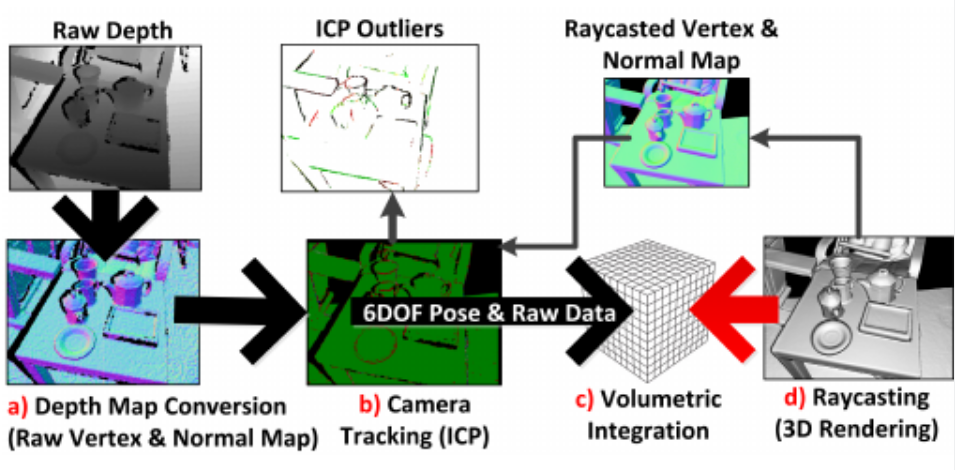
\includegraphics[width=0.66\textwidth, frame]{images/kinfu-integration.png}
	\caption{Integration eines Tiefenbilds in \ac{KinFu}. Entnommen aus \cite{izadi2011kinectfusion}}
	\label{fig:kinfu-integration}
\end{figure}

Durch eine schnelle GPU-Implementierung auf Basis von CUDA erreicht \ac{KinFu} dabei eine Integration neuer Tiefenbilder bei 30 Hz, der Bildwiederholfrequenz der Kinect.
Somit ist die zeitliche Differenz zwischen zwei Aufnahmen sehr niedrig.
Es wird davon ausgegangen, dass die Kamera handgeführt (bzw. mit geringer Geschwindigkeit bewegt) wird.
Daher hält sich auch die räumliche Distanz zwischen einzelnen Frames in Grenzen.
Aufgrund dieser Gegebenheiten reicht bei \ac{KinFu} eine lokale Registrierung aus, es kann also direkt \ac{ICP} verwendet werden.

In \autoref{fig:kinfu-integration} ist der Ablauf der Integration eines neuen Tiefenbilds ins \ac{TSDF} bei \ac{KinFu} dargestellt.
Das Tiefenbild wird zunächst in eine Punktwolke konvertiert.
Diese wird anschließend durch \ac{ICP} registriert, um dann unter Bildung eines Mittelwerts in das \ac{TSDF} integriert zu werden.
Zur Darstellung der Szene wird dieses anschließend mithilfe eines Raycasters gerendert.


Es gibt zahlreiche Optimierungen und veränderte Versionen von \ac{KinFu}.
Unter anderem gibt es in der \ac{PCL} eine freie Implementierung \cite{pirovano2012kinfu}.
Eine optimierte Version ist beispielsweise Chisel \cite{klingensmith2015chisel}, bei der eine effizientere Voxelstrategie verwendet wird.
Weiterhin ist Chisel eine reine CPU-Implementierung, was die Nutzung auf Mobilgeräten ohne Grafikkarte ermöglicht.

Die in dieser Arbeit verwendete Implementierung ist \ac{YAK}.
\ac{YAK} ist eine auf \ac{ROS} angepasste Version von \ac{KinFu}, um Trajectory Waypoints für die Robotersteuerung zu errechnen \cite{schornak2019yak}.
Die Verwendung von \ac{KinFu} in industriellen Robotikanlagen ist in vielerlei Hinsicht sinnvoll:
\begin{itemize}
\item Objekte können aus mehreren Perspektiven gescannt werden, was eine bessere Darstellung der Szene liefert.
\item Rauschen durch den Bildsensor wird aufgrund der Mittelwertbildung minimiert.
Das Ergebnis ist ein glatteres und realistischeres Modell.
\item Durch die GPU-Implementierung können Tiefenbilder in Echtzeit integriert werden, was insbesondere bei Robotikanwendungen ein großer Vorteil ist.
\item Ein häufig in der Bildverarbeitung auftretendes Problem sind reflektierende bzw. spiegelnde Oberflächen.
Die betroffenen Regionen können oft nur falsch, verzerrt oder gar nicht modelliert werden.
Da hier eine Aufnahme aus mehreren Perspektiven möglich ist, können derartige Fehler weitestgehend vermieden werden. In \autoref{fig:yak-reflecting-model} ist dies an einem Beispiel besonders gut sichtbar.
\end{itemize}

\begin{figure}[H]
	\centering
	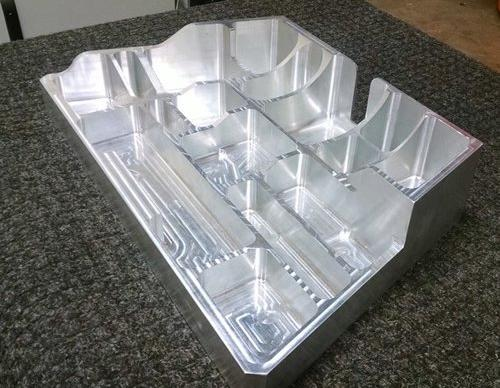
\includegraphics[width=0.4\textwidth]{images/yak-reflecting-scene.jpg}
	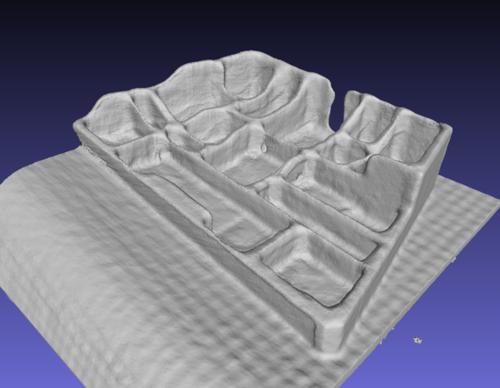
\includegraphics[width=0.4\textwidth]{images/yak-reflecting-reconstruction.png}
	\caption{Szene und Rekonstruktion eines reflektierenden Objekts durch \ac{YAK}. Entnommen aus \cite{schornak2019yak}}
	\label{fig:yak-reflecting-model}
\end{figure}

Der Vorteil der Echtzeitintegration ist jedoch gleichzeitig auch ein großes Problem.
In industriellen Robotikanlagen sind nur selten Grafikkarten verbaut.
Eine Hochleistungs-GPU-Einheit ist dabei aber unerlässlich, da sonst nur ein Bruchteil der Geschwindigkeit erreicht werden kann.
Weiterhin ist CUDA ein proprietäres Softwarepaket, was die Nutzung mit Grafikkarten von anderen Herstellern unmöglich macht.



\section{Triangulierung}
\label{sec:triangulation}

Die Konvertierung von punktbasierten Objektinformationen zu einem aus zusammenhängenden Dreiecken bestehenden Mesh nennt sich Triangulierung.
Gerade bei der Triangulierung von Punktwolken ist eine eindeutige korrekte Lösung dieses Problems jedoch häufig nicht vorhanden.
Es ist beispielweise nicht immer sichergestellt, dass jeder Punkt auch tatsächlich die zu rekonstruierende Oberfläche darstellt -- Rauschen, Reflektionen oder sonstige Fehler können auftreten.
Weiterhin stellt sich die Frage, aus welchen der Punkten in der Wolke sich ein bestimmtes Polygon zusammensetzt.

Diese und andere Probleme führen dazu, dass es viele verschiedene Ansätze zur Triangulierung gibt.


\subsection{Marching Cubes}
\label{subsec:marching-cubes}

Bei Marching Cubes \cite{lorensen1987marching} handelt es sich um einen Algorithmus, der ursprünglich zur Triangulierung medizinischer Computertomographiescans entwickelt wurde.
Diese werden in den meisten Fällen als Voxel Grid dargestellt.
Für die Anwendung auf einer Punktwolke muss diese also zunächst konvertiert werden.
Der Ablauf ist in \autoref{alg:marching-cubes} beschrieben.

Das Ziel des Algorithmus ist es, die sogenannte Isofläche aus den 3D-Daten zu extrahieren, welche dann durch die einzelnen Dreiecke approximiert wird.
Die Isofläche repräsentiert im Falle einer Punktwolke die Oberfläche eines Objekts.
Die Punkte liegen also bei fehlerfreien Daten exakt darauf.
Um festzulegen, ab wann ein Punkt innerhalb der Oberfläche gesehen wird, muss sein Wert unter dem Parameter $\alpha$ liegen.

Die eingegebene Punktwolke wird also zunächst diskretisiert, was bei geringer Kantenlänge der Voxel zu Datenverlust führt.
Anschließend wird jeder Voxel getrennt betrachtet und anhand der Eckkonfiguration die zu verbindenden Kanten mithilfe einer Lookup Table ermittelt.
Dieses Vorgehen wird nun für jeden Voxel wiederholt, was zu einer vollständigen Rekonstruktion der Oberfläche führt.

\begin{algorithm}[H]
\caption[Marching Cubes]{Marching Cubes \cite[Abs. 4]{lorensen1987marching}}
\label{alg:marching-cubes}
\begin{algorithmic}
\State $\mathcal{L} \gets \emptyset$
\Comment{The list of output vertices (Faces implicit)}
\State $\mathcal{V} \gets Voxels$
\ForAll{$v \in \mathcal{V}$}
	\State $i \gets$ \Call{calculateIndex}{$v$}
	\State $\mathcal{E} \gets edgeTable[i]$
	\ForAll{$e \in \mathcal{E}$}
		\State $p \gets$ \Call{interpolate}{$e[0], e[1]$}
		\Comment{interpolate corners}
		\State \Call{$\mathcal{L}$.add}{$p$}
	\EndFor
\EndFor
\State \Return{$\mathcal{L}$}
\Function{calculateIndex}{$v$}
	\State $x \gets 0$
	\For{$corner \in \{0, \dots, 7\}$}
		\If{$v[corner] < \alpha$}
		\Comment{corner inside isosurface}
			\State $x\ |=\ 1 << corner$
			\Comment{Set the i-th bit to $1$}
		\EndIf
	\EndFor
	\State \Return{$x$}
\EndFunction
\end{algorithmic}
\end{algorithm}

Einer der entscheidenden Nachteile bei diesem Algorithmus ist, dass die Qualität des Meshs direkt abhängig von der gewählten Kantenlänge der Voxel ist.
Dies macht viele Vorteile der Punktwolke gegenüber einem Voxel Grid zunichte.
Bei zu geringer Kantenlänge nimmt die Zahl der möglichen rekonstruierten Polygone ab, was zu einer geringeren Qualität führt.

Wählt man die Auflösung jedoch zu hoch, treten Oversampling-Effekte auf und es entstehen Lücken im Mesh.
Insbesondere bei großen Differenzen der Distanzen zwischen Punkten in der Punktwolke führt dies zu Problemen.
Insgesamt kann bei Marching Cubes die Topologie des Objekts verfälscht dargestellt werden \cite[2]{chernyaev1995marching}.

Weiterhin weisen die Meshes in der Standardimplementierung zackenartige Artefakte auf.
Dies passiert dann, wenn die Vertices zu den entsprechenden Kanten mittig auf diesen gewählt werden.
Durch eine Interpolation zwischen den Werten der beiden Eckpunkte des Voxels lässt sich dieser Effekt minimieren.


\subsection{Poisson}
\label{subsec:poisson}

Die \citeyear{kazhdan2006poisson} von \citeauthor{kazhdan2006poisson} präsentierte Poisson-Rekonstruktion \cite{kazhdan2006poisson} basiert auf der impliziten Darstellung der Oberfläche als Funktion.
Die mathematische Darstellung dieser Funktion lässt sich \autoref{def:poisson-surface} entnehmen.

\begin{definition}
\label{def:poisson-surface}
Sei $M$ die zu rekonstruierende Oberfläche.
Dann ist
\begin{equation}
\chi_M(p) = \left\{
\begin{array}{ll}
0 & p\ \mathrm{außerhalb\ von}\ M\\
1 & p\ \mathrm{innerhalb\ von}\ M\\
\end{array}
\right.
,\ \forall q \in M : \chi_M(q) = 0.5
\end{equation}
die implizite Funktion, die die Oberfläche im Punkt $p \in M$ darstellt.
\end{definition}

Der Gradient $\nabla \chi_M$ dieser Funktion nimmt also im optimalen Fall überall den Wert $0$ an, außer in der Oberfläche selbst.
Dieser Gradient entspricht exakt den nach innen gerichteten Normalen in den Oberflächenpunkten \cite[Abs. 3]{kazhdan2006poisson}.
Somit gilt für die Indikatorfunktion:

\begin{displaymath}
\begin{aligned}
&&\nabla \chi_M && = &&\overrightarrow{V}\\
\Leftrightarrow && \nabla^2 \chi_M && = &&\nabla \overrightarrow{V}\\
\Leftrightarrow && \Delta \chi_M && = &&\nabla \overrightarrow{V}
\end{aligned}
\end{displaymath}

Dies ist eine Poisson-Gleichung \cite[Kap. 2]{ponce2016pde}, deren Lösung sich beispielsweise mit dem Gauß-Seidel-Verfahren iterativ berechnen beziehungsweise annähern lässt.
Da eine genaue Lösung der Poissongleichung nur in der Nähe der Oberfläche erforderlich ist, kann nun ein Octree aufgestellt werden.

Mit der Poisson-Rekonstruktion generierte Polygonmeshes weisen die Eigenschaft auf, immer wasserdicht zu sein.
Dies ist in der Darstellung der Oberfläche als mehrdimensionale, kontinuierliche Funktion begründet.

Die Auflösung des Meshes lässt sich durch die maximale Baumtiefe einstellen.
Mit der Tiefe und damit der Qualität steigen jedoch auch Laufzeit und Speicherbedarf drastisch an.
Weiterhin kann konfiguriert werden, wie viele Punkte einem Blatt im Baum zugewiesen werden.
Hohe Werte führen zu einer verringerten Auflösung, aber auch zu einem gleichzeitigen Glättungseffekt.
Außerdem verringern sich aufgrund der niedrigeren Zahl an Blättern der benötigte Speicher und die Laufzeit.


\subsection{Weitere Ansätze}
\label{subsec:triangulation-others}

Neben den bereits genannten Rekonstruktionsalgorithmen Marching Cubes und Poisson gibt es noch weitere unterschiedliche Ideen, um ein Polygonnetz zu triangulieren.

\subsubsection{Greedy-Triangulierung}
\label{subsubsec:greedy-triangulierung}

Bei der Greedy-Triangulierung der Wolke $\mathcal{P}$ werden zunächst alle Punkte $p, q \in \mathcal{P}$ miteinander verknüpft.
So entstehen Kantenkandidaten, welche nun nach ihrer Länge sortiert werden.
Diese werden nun nacheinander akzeptiert oder verworfen, wenn ein Schnittpunkt mit einer bereits akzeptierten Kante auftritt \cite[235--237]{preparata1985computational}.

\begin{algorithm}[H]
\caption{Greedy-Triangulierung}
\label{alg:greedy-triangulierung}
\begin{algorithmic}
\State $\mathcal{C} \gets \emptyset$
\ForAll{$p, q \in \mathcal{P},\ p \neq q$}
\Comment{add edge candidates to $\mathcal{C}$}
	\State \Call{add}{$\mathcal{C}$, $\overline{pq}$}
\EndFor
\State \Call{sortByLength}{$\mathcal{C}$}
\State $\mathcal{T} \gets \emptyset$
\Comment{the accepted edges}
\ForAll{$e \in \mathcal{C}$}
	\ForAll{$f \in \mathcal{T}$}
		\If{$e \cap f$}
		\Comment{$e$ intersects $f$, remove from candidates}
			\State $\mathcal{C} \gets \mathcal{C} \setminus \{e\}$
		\EndIf
	\EndFor
	\State $\mathcal{T} \gets \mathcal{T} \cup \{e\}$
\EndFor
\State \Return{$\mathcal{T}$}
\end{algorithmic}
\end{algorithm}

Diese Art der Triangulierung funktioniert nur im zweidimensionalen Raum, da der Schnittpunkt zwischen zwei Geraden in höheren Dimensionen nicht als Kriterium ausreicht.
Im $\mathbb{R}^3$ werden daher die Punkte über ihre Normale auf eine Ebene projeziert.
Zur Anwendung auf 3D-Punktwolken ist daher eine vorherige Normalenschätzung notwendig.
Anschließend kann der in \autoref{alg:greedy-triangulierung} dargestellte Ablauf regulär durchgeführt werden.

Ein enormer Vorteil der Greedy-Triangulierung ist ihre Geschwindigkeit.
So zeigen \citeauthor{berg2000comp}, dass ein Polygon mit $n$ Vertices in $\mathcal{O}(n \log n)$ rekonstruiert werden kann \cite[56--58]{berg2000comp}.
Dies ist beispielsweise für Echtzeitanwendungen relevant, wie die in \cite{Marton09ICRA} vorgestellte Methode demonstriert.

\subsubsection{Delaunay-Triangulierung}
\label{subsubsec:delaunay-triangulierung}

Dreiecke mit mindestens einem kleinen Innenwinkel sind häufig problematisch in der Computergrafik.
Beim Renderingprozess können aufgrund von Präzisions- und Rundungsfehlern Artefakte und Aliasingeffekte auftreten.

Die Delaunay-Triangulierung behebt dieses Problem weitestgehend, da sie die minimalen Innenwinkel der generierten Dreiecke maximiert \cite[199]{berg2000comp}.
Eine weitere Eigenschaft ist, dass kein Umkreis eines der Dreiecke einen Knoten beinhaltet, der nicht eine Ecke des Dreiecks ist \cite[196]{berg2000comp}. Der Ablauf der Delaunay-Triangulierung ist in \autoref{alg:delaunay-triangulierung} zu sehen.

\begin{algorithm}[H]
\caption[Delaunay-Triangulierung]{Delaunay-Triangulierung \cite[200--201]{berg2000comp}}
\label{alg:delaunay-triangulierung}
\begin{algorithmic}
\State $\mathcal{P} \gets$ list of $n$ vertices $p_1, \dots, p_n$
\State $\mathcal{T} \gets$ a triangle $p_0 q r$ with $p_0 \in \mathcal{P}$ so that $\forall p \in \mathcal{P} : p \mathrm{\ inside\ } p_0 q r$
\State $\mathcal{P} \gets \mathcal{P} \setminus \{p_0\}$
\While{$\mathcal{P} \neq \emptyset$}
	\State $p_r \gets$ \Call{$\mathcal{P}$.pop()}{}
	\State find triangle $t \in \mathcal{T}$ so that $p_r$ is inside $t$
	\State $\mathcal{T} \gets \mathcal{T} \setminus \{t\}$
	\If{$p_r$ is on edge $t_1t_2 \in t$}
		\State find vertices $v_1$ and $v_2$ of the two triangles seperated by $t_1t_2$
		\State create triangles $t_1p_rv_1$, $t_1v_2p_r$, $t_2v_1p_r$ and $t_2p_rv_2$
		\State check the untouched edges using \Call{checkFlipped}{$p_r$, edge}
		\State add the triangles to $\mathcal{T}$
	\Else
		\State $p_r$ is inside $t = t_1t_2t_3$
		\State split $t$ into three triangles with $p_r$ as vertex
		\State check the old edges using \Call{checkFlipped}{$p_r$, edge}
		\State add them to $\mathcal{T}$
	\EndIf
	\State remove all triangles $t \in \mathcal{T}$ which have $q$ or $r$ as vertex
\EndWhile
\State \Return{$\mathcal{T}$}

\Function{checkFlipped}{new vertex $p$, edge $t$}
	\If{the smallest angle is bigger after a flip}
		\State get two triangles $a, b \in \mathcal{T}$ separated by $t$
		\State connect vertices $p_1 \in a$ and $p_2 \in b$ not connected by $t$
		\State remove $t$
		\State check old edges not ending at $p$ using \Call{checkFlipped}{$p$, edge}
	\EndIf
\EndFunction
\end{algorithmic}
\end{algorithm}

\subsubsection{Ball Pivoting}
\label{subsubsection:ball-pivoting}

Die Ball-Pivoting-Rekonstruktion liefert eine sehr anschauliche und intuitive Möglichkeit, eine Punktwolke zu triangulieren.
Dabei wird ein imaginärer Ball mit Radius $\rho$ auf ein Seed-Dreieck gelegt und nacheinander über die Kanten gerollt \cite{bernardini1999ball}.
Trifft er dabei auf einen weiteren Punkt, wird aus diesem und der bereits existierenden Kante ein neues Dreieck gebildet.
Falls er auf keinen Punkt trifft, handelt es sich um eine Außenkante, die nicht weiter betrachtet wird.
Der genaue Ablauf ist in \autoref{alg:ball-pivoting} dargestellt.

\begin{algorithm}[H]
\caption[Ball Pivoting]{Ball Pivoting \cite[Abs. 4]{bernardini1999ball}}
\label{alg:ball-pivoting}
\begin{algorithmic}
\State $\rho \gets$ the ball radius
\State $\mathcal{F} \gets$ seed triangle
\While{true}
	\While{$e_{(i,j)} \gets$ \Call{getActiveEdge}{$\mathcal{F}$}}
		\If{$\sigma_k \gets$ \Call{ballPivot}{$e_{(i,j)}$} $\wedge\ ($\Call{notUsed}{$\sigma_k$} $\vee$ \Call{onFront}{$\sigma_k$}$)\ $}
			\State \Call{outputTriangle}{$\sigma_i$, $\sigma_k$, $\sigma_j$}
			\State \Call{join}{$e_{(i,j)}$, $\sigma_k$, $\mathcal{F}$}
			\If{$e_{(k,i)} \in \mathcal{F}$}
				\State \Call{glue}{$e_{(i,k)}$, $e_{(k,i)}$, $\mathcal{F}$}
			\EndIf
			\If{$e_{(j,k)} \in \mathcal{F}$}
				\State \Call{glue}{$e_{(k,j)}$, $e_{(j,k)}$, $\mathcal{F}$}
			\EndIf
		\Else
			\State \Call{markAsBoundary}{$e_{(i,j)}$}
		\EndIf
	\EndWhile
	\If{$(\sigma_i, \sigma_j, \sigma_k) \gets$ \Call{findSeedTriangle()}{}}
		\State \Call{outputTriangle}{$\sigma_i$, $\sigma_j$, $\sigma_k$}
		\State \Call{insertEdge}{$e_{(i,j)}$, $\mathcal{F}$}
		\State \Call{insertEdge}{$e_{(j,k)}$, $\mathcal{F}$}
		\State \Call{insertEdge}{$e_{(k,i)}$, $\mathcal{F}$}
	\Else
		\State \Return
	\EndIf
\EndWhile
\end{algorithmic}
\end{algorithm}

Ein Nachteil des Ball-Pivoting-Algorithmus ist, dass bei zu groß gewählten Radien einige Details verloren gehen können.
Dies tritt insbesondere dann auf, wenn die rekonstruierte Oberfläche stark konkav ist und die Abstände zwischen den Punkten deutlich kleiner als der gewählte Radius sind.

Um diesem Fall vorzubeugen, kann man mehrere Triangulierungen mit unterschiedlichen Werten für $\rho$ kombinieren.
Aufgrund der mehrfachen Ausführung führt dies jedoch zu einer deutlich erhöhten Laufzeit.